\documentclass[border=6pt]{standalone}
\usepackage{tikz}
\usetikzlibrary{arrows.meta,positioning}
\begin{document}
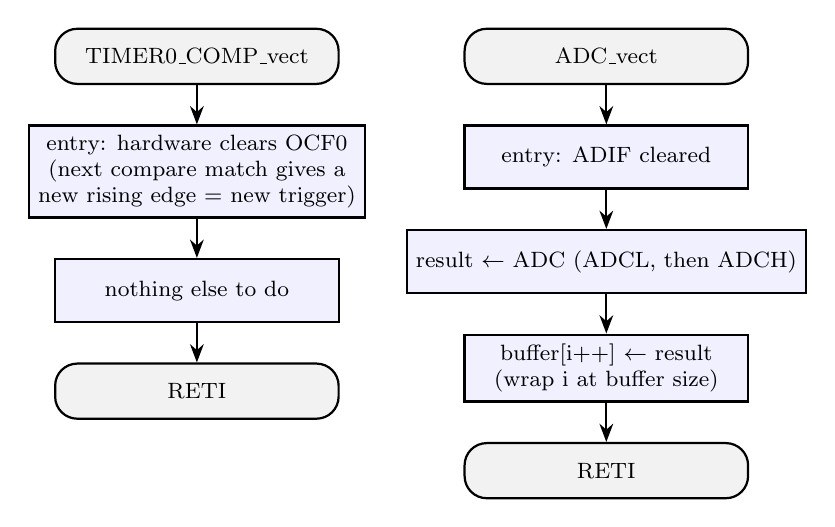
\begin{tikzpicture}[>=Stealth,font=\small,node distance=0.5cm,
 term/.style={draw,thick,rounded corners=8pt,fill=gray!10,minimum width=3.6cm,minimum height=0.7cm,align=center,font=\footnotesize},
 proc/.style={draw,thick,fill=blue!6,minimum width=3.6cm,minimum height=0.8cm,align=center,font=\footnotesize}]
\node[term] (a0) {TIMER0\_COMP\_vect};
\node[proc,below=of a0] (a1) {entry: hardware clears OCF0\\(next compare match gives a\\new rising edge = new trigger)};
\node[proc,below=of a1] (a2) {nothing else to do};
\node[term,below=of a2] (a3) {RETI};
\draw[->,thick] (a0) -- (a1); \draw[->,thick] (a1) -- (a2); \draw[->,thick] (a2) -- (a3);
\begin{scope}[xshift=5.2cm]
\node[term] (b0) {ADC\_vect};
\node[proc,below=of b0] (b1) {entry: ADIF cleared};
\node[proc,below=of b1] (b2) {result $\leftarrow$ ADC (ADCL, then ADCH)};
\node[proc,below=of b2] (b3) {buffer[i++] $\leftarrow$ result\\(wrap i at buffer size)};
\node[term,below=of b3] (b4) {RETI};
\draw[->,thick] (b0) -- (b1); \draw[->,thick] (b1) -- (b2); \draw[->,thick] (b2) -- (b3); \draw[->,thick] (b3) -- (b4);
\end{scope}
\end{tikzpicture}
\end{document}
